\documentclass{article}
\linespread{1.3}
\usepackage[margin=50pt, headheight=60pt, headsep=0pt]{geometry}
\usepackage{amsmath, amssymb, amsthm, tikz, fancyhdr, float, graphicx, spverbatim, systeme}
\pagestyle{fancy}
\renewcommand{\headrulewidth}{0pt}
\newcommand{\changefont}{\fontsize{15}{15}\selectfont}

\fancypagestyle{firstpageheader}{
  \fancyhead[R]{
    \changefont
    \parbox[t]{4cm}{ % Adjust width as needed
      Michael Huang\\
      EN.625.740.81\\
      Homework 8
    }
  }
}

\begin{document}

\thispagestyle{firstpageheader}
{\Large 

\section*{1.}


}
{\Large 

\section*{2.}
Given data \((X_1, Y_1), \dots, (X_n, Y_n)\), consider the regression through the origin model
\[
  Y_i = \beta X_i + v_i, 
\]
where \(E(v_i | X_i) = 0\) and \(\text{Var}(v_i | X_i) = \sigma^2\).

\subsection*{(a)} 
Find \(\hat{\beta}\), the least squares estimate for \(\beta\). \\ \\


\subsection*{(b)}
Find the standard error of the estimate, \(\sqrt{\text{Var}(\hat{\beta}).}\) \\ \\


\subsection*{(c)}
Find conditions that guarantee that the estimate is consistent: 
\[
  \forall \epsilon > 0, P(|\hat{\beta} - \beta| > \epsilon) \to 0 \text{ as } n \to \infty.
\] \\


}
{\Large 

\section*{3.}
The columns in the file \texttt{polynomial\_data.txt} are the \(X\) and \(Y\) values of a polynomial function \(y = \sum_{k=0}^{n} a_k x^k\) with added Gaussian noise. 

\subsection*{(a)} 
For each \(n \in \{3, 4, 5, 6\}\), fit an \(n^{\text{th}}\) degree polynomial to the data. What would you say is the most likely value of \(n\)? \\ \\
I ran the Python script below and got the following output:
\begin{spverbatim}
> python problem_3.py
            rss        rse  adj_r_2
n                                  
3  1.122068e+07  341.88019  0.96305
4  1.121543e+07  343.59444  0.96268
5  3.232150e+06  185.43078  0.98913
6  3.212240e+06  185.84997  0.98908
\end{spverbatim}
From this, it seems that \(n = 5\) is a good fit since the RSS, RSE and R squared all stop significantly improving around then. We can also check by plotting to see about the fit, which looks pretty good:
\begin{figure}[h!]
  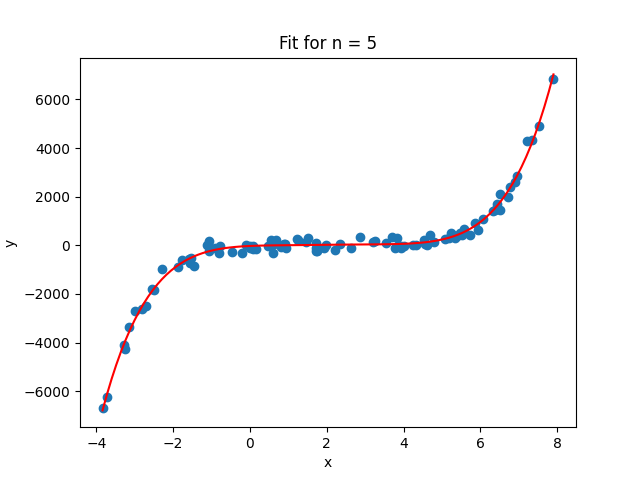
\includegraphics[width=400pt]{problem_3_a_plot.png}
\end{figure} \\ 
This is the corresponding Python code:
\begin{spverbatim}
import matplotlib.pyplot as plt
import numpy as np
import pandas as pd
import statsmodels.api as sm

data = np.loadtxt("polynomial_data.txt")

N_VALUES = [3, 4, 5, 6]

x_data = data[:, 0]
y_data = data[:, 1]

def poly_function(x_data, n):
  """Build the corresponding matrix by stacking 1, x, x^2, etc."""
  return np.column_stack(
    [x_data**k for k in range(n + 1)]
  )

fit_results = []
result_summaries = []

for n in N_VALUES:
  fit_result = sm.OLS(y_data, poly_function(x_data, n)).fit()
  fit_results.append(fit_result)

  result_summaries.append({
    "n": n,
    "rss": fit_result.ssr,
    "rse": np.sqrt(fit_result.scale),
    "adj_r_2": fit_result.rsquared_adj,
  })

result_summary_df = pd.DataFrame(result_summaries).set_index("n").round(5)
print(result_summary_df)

# n = 5 seems good enough, so plot and see
plt.scatter(x_data, y_data)
x_series = np.linspace(min(x_data), max(x_data), 100)
# Index 2 in fit_results since n_values = [3, 4, 5, 6]
plt.plot(x_series, fit_results[2].predict(poly_function(x_series, 5)), color="red")
plt.xlabel("x")
plt.ylabel("y")
plt.title("Fit for n = 5")
plt.show()
\end{spverbatim}

\subsection*{(b)}
Estimate the level of the noise. \\ \\
The output from my script was as follows:
\begin{spverbatim}
Estimated noise standard deviation: 185.43077663414547
Estimated noise variance: 34384.572923142354
\end{spverbatim}
This was from the following block of code at the bottom of my python script:
\begin{spverbatim}
# Print RSE as noise estimation for n = 5
sigma = np.sqrt(fit_results[2].scale)
print(f"Estimated noise standard deviation: {sigma}")
print(f"Estimated noise variance: {sigma**2}")
\end{spverbatim}
Looking at our table in part (a), the RSE values stabilize significantly once the model complexity reaches \(n=5\). I chose to use RSE as a measure of noise used as established in the text. Comparing this noise to the plot and the mean values of \(y\), it seems that this RSE with standard deviation of approximately 185 is relatively low compared to the \(y\)-values in the thousands.

}
{\Large 

\section*{4.}
Let \(r = \text{Cor}(X, Y)\) in equation (3.18) on page 70 of \textbf{An Introduction to Statistical Learning with R}, Second Edition. Show that for simple linear regression, \(R^2 = r^2\). \\ \\

}

\end{document}